% ============================================================================
% Section 2: Axioms — From Phenomenal Properties to Physical Postulates
% ============================================================================

\section{From phenomenal properties to physical postulates}
\label{sec:axioms}

Like IIT~\cite{iit4}, UHM begins with properties of experience and translates them into
mathematical postulates. Unlike IIT, UHM's postulates are grounded in a specific algebraic
structure (octonions) and a specific combinatorial structure (Fano plane), which uniquely
determine the dimensionality and architecture of the theory. UHM rests on \textbf{four axioms} (A1--A4), all of which are now themselves derived
as theorems (see Section~\ref{subsec:cohesive-closure} and below); a fifth axiom (A5,
Page--Wootters temporal constraint) is \emph{derived} from A1--A4 via the spectral triple
construction (T-87~\status{T}).

\subsection{The single primitive}

\begin{axiombox}[Axiom of Omega]
The only primitive of the theory is the $\infty$-topos of sheaves on the site of density
matrices:
\begin{equation}
  \mathfrak{T} := \bigl(\ShInf(\mathcal{C}),\; J_{\mathrm{Bures}},\; \omega_0\bigr)
\end{equation}
where $\mathcal{C} = \mathbf{DensityMat}(\mathbb{C}^7)$ is the category of $7 \times 7$
density matrices, $J_{\mathrm{Bures}}$ is the Grothendieck topology induced by the Bures
metric, and $\omega_0$ is the subobject classifier.
\end{axiombox}

Everything else --- spacetime, quantum mechanics, gravity, consciousness --- is derived, not
postulated. The coherence matrix $\Gam$ is an object of this category:
$\Gam \in \mathrm{Ob}(\mathcal{C})$.

\subsubsection*{The four axioms (all derived)}

\begin{enumerate}[leftmargin=2em]
  \item \textbf{(A1) Structure \status{T}:} Reality is an $\infty$-topos $\ShInf(\mathcal{C})$ over
        the site of density matrices $\Dens(\mathbb{C}^7)$, generating continuous CPTP
        dynamics $\Lind_\Omega$ (Lindbladian form via GKSL theorem).
  \item \textbf{(A2) Metric \status{T}:} The Grothendieck topology $J_{\mathrm{Bures}}$ is induced
        by the Bures distance:
        \begin{equation}
          d_B(\Gam, \Gam') = \sqrt{2 - 2\sqrt{F(\Gam, \Gam')}}
          \label{eq:bures}
        \end{equation}
        where $F(\Gam, \Gam') = \bigl(\Tr\sqrt{\sqrt{\Gam}\,\Gam'\sqrt{\Gam}}\,\bigr)^2$
        is the Uhlmann fidelity. By the Petz classification~\cite{petz1996}, the Bures metric is the
        \emph{minimal} monotone Riemannian metric on $\Dens(\Hil)$
        (in the classical case, the Fisher metric is unique by
        Chentsov's theorem~\cite{chentsov1982}; in the quantum case,
        infinitely many monotone metrics exist, but Bures is minimal).
        This choice ensures $\Pcrit = 2/7$ is the least restrictive threshold.
        \emph{Derived status:} T-187 proves that Bures is the uniquely canonical
        Petz-enrichment, fixed by three independent characterizations (Petz extremality,
        Uhlmann purification, SLD-Fisher saturation), making A2 a theorem rather
        than a postulate (Section~\ref{subsec:cohesive-closure}).
  \item \textbf{(A3) Dimension \status{T}:} The base Hilbert space dimension is $N = 7$, grounded
        in octonion structure $G_2 = \mathrm{Aut}(\Oct)$ and the Fano plane $\Fano$
        (Section~\ref{subsec:why-seven}).
  \item \textbf{(A4) Scale \status{T}:} Characteristic frequency
        $\omega_0 = \lambda_{\min}(H_{\mathrm{eff}}) > 0$ relates internal time $\tau$ to
        physical time $t$. This is not a free parameter: $\omega_0$ is the minimal nonzero
        eigenvalue of the effective Hamiltonian $H_{\mathrm{eff}}$ (T-87). A system with
        $\omega_0 = 0$ has no dynamics, hence no regeneration, hence is not viable. Different
        holons have different $\omega_0$, just as different atoms have different masses ---
        a computed spectral property, not a postulated one.
\end{enumerate}

From these four, a fifth constraint is derived (T-87~\status{T}):

\begin{enumerate}[leftmargin=2em, start=5]
  \item \textbf{(A5, derived) Page--Wootters temporal constraint~\cite{page1983}:}
        $[\hat{C},\, \Gam_{\mathrm{total}}] = 0$, yielding emergent time from the
        O-dimension (Section~\ref{subsec:emergent-time}).
\end{enumerate}

\paragraph{Principle of Informational Distinguishability (PID, T-16~\status{T}).}
Given A1 and A2, a further principle follows tautologically: two states are ontologically
distinct if and only if they are distinguishable by $J_{\mathrm{Bures}}$-coverings. This
connects the mathematical formalism to consciousness: subjective distinctness and physical
distinguishability are the same relation. PID is not an additional axiom --- it is a
consequence of taking A1 and A2 seriously~\status{O}.

The Bures metric on $\Dens(\mathbb{C}^7)$ defines a topology in the point-set sense. This topology generates a Grothendieck site: coverings are families of open inclusions that jointly cover an open set. By Lurie's theorem (HTT 6.2.2.7), the $\infty$-category of sheaves on this site is an $\infty$-topos, provided the Giraud axioms (descent, universal colimits, disjoint coproducts, effective groupoid objects) are satisfied. For the site of density matrices with the Bures topology, these axioms hold by construction~\cite{lurie2009}. The site axioms (identity, stability under pullback, transitivity) are verified via CPTP contractivity of the Bures metric (Uhlmann 1976) and the essentially small presentation of the compact metrizable $\Dens(\mathbb{C}^7)$ (Johnstone, \emph{Elephant} C2.1.9--12).

\textbf{Why Bures specifically?} T-187~\status{T} provides \emph{three logically
independent} mathematical witnesses plus \emph{one physical recasting}: (Char-I)~Petz
extremality (minimal in the Petz poset), (Char-II)~Uhlmann purification universality,
(Char-III)~SLD-Cram\'{e}r--Rao saturation, plus (Char-IV, T-189~\status{T})~a
\emph{physical selector} $g^{ij} = C^{ij}_{\mathrm{SLD}}$ matching the inverse metric
against the Petz-free SLD covariance (defined from
$\partial\rho = \tfrac12(L_i\rho + \rho L_i)$ without reference to any metric). Char-IV
reduces to Char-III via $g_B^{-1} = C_{\mathrm{SLD}}$ (Braunstein--Caves 1994), so it is
not a fourth logically independent witness --- it is a statistical-mechanical recasting
that strengthens the physical motivation of T-187 without adding mathematical redundancy.
T-187 retains status \status{T} on the strength of Char-I (Petz extremality) alone.

\textbf{Why $\infty$-topos?}~\cite{lurie2009} An $\infty$-topos provides three things simultaneously:
(1)~an internal logic (Heyting algebra, not Boolean --- capturing the fact that propositions
about consciousness need not satisfy the law of excluded middle);
(2)~a notion of ``space'' (Bures metric on density matrices, from which physical spacetime
emerges); (3)~higher morphisms at all levels (allowing self-reference without paradox,
via Lawvere's fixed-point theorem). No simpler structure provides all three.

\subsection{Why seven dimensions: the Fano plane and octonions}
\label{subsec:why-seven}

The number 7 is not chosen --- it is \emph{derived}. Two independent mathematical arguments
converge on the same value.

\paragraph{Argument 1: Octonion algebra.}
The octonions $\Oct$ form the unique normed division algebra in 8 dimensions (by the
Hurwitz theorem~\cite{hurwitz1898}, the only normed division algebras are $\mathbb{R}$,
$\mathbb{C}$, $\mathbb{H}$, and $\Oct$). The imaginary part of $\Oct$ has dimension 7:
$\dim(\mathrm{Im}(\Oct)) = 7$. The automorphism group of $\Oct$ is the exceptional
Lie group $G_2$, which has dimension 14.

\paragraph{Argument 2: Fano plane $\Fano$.}
The Fano plane is the smallest finite projective plane: 7 points and 7 lines,
where each line passes through exactly 3 points, and each point lies on
exactly 3 lines (Figure~\ref{fig:fano}). It is the incidence geometry of
the octonion multiplication table.

\begin{figure}[H]
\centering
% Fano Plane PG(2,2) — The Architecture of Self-Observation
% 7 points = 7 dimensions, 7 lines = 7 observation triples

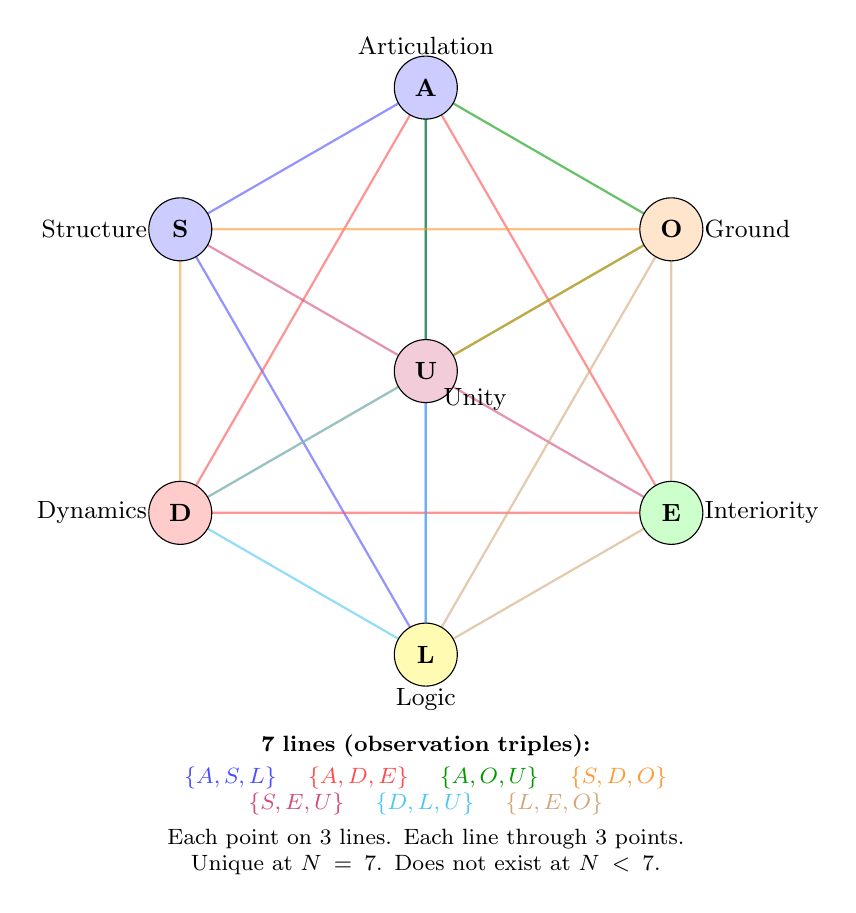
\begin{tikzpicture}[
  point/.style={circle, fill=#1, draw=black, minimum size=8mm, inner sep=0pt, font=\small\bfseries},
  line/.style={thick, #1},
  scale=1.8
]

% === Coordinates (regular hexagon + center) ===
\coordinate (A) at (90:2);     % top
\coordinate (S) at (150:2);    % upper-left
\coordinate (D) at (210:2);    % lower-left
\coordinate (L) at (270:2);    % bottom
\coordinate (E) at (330:2);    % lower-right
\coordinate (O) at (30:2);     % upper-right
\coordinate (U) at (0:0);      % center

% === Lines (7 Fano lines, drawn first so points overlay) ===
% Line 1: {A, S, L}
\draw[line=blue!70, opacity=0.6] (A) -- (S) -- (L) -- cycle;
% Line 2: {A, D, E}
\draw[line=red!70, opacity=0.6] (A) -- (D) -- (E) -- cycle;
% Line 3: {A, O, U}
\draw[line=green!60!black, opacity=0.6] (A) -- (O) -- (U) -- cycle;
% Line 4: {S, D, O}
\draw[line=orange!80, opacity=0.6] (S) -- (D) -- (O) -- cycle;
% Line 5: {S, E, U}
\draw[line=purple!70, opacity=0.6] (S) -- (E) -- (U) -- cycle;
% Line 6: {D, L, U}
\draw[line=cyan!70, opacity=0.6] (D) -- (L) -- (U) -- cycle;
% Line 7: {L, E, O} — the inscribed circle line
\draw[line=brown!70, opacity=0.6] (L) -- (E) -- (O) -- cycle;

% === Points ===
\node[point=blue!20]   at (A) {A};
\node[point=blue!20]   at (S) {S};
\node[point=red!20]    at (D) {D};
\node[point=yellow!30] at (L) {L};
\node[point=green!20]  at (E) {E};
\node[point=orange!20] at (O) {O};
\node[point=purple!20] at (U) {U};

% === Labels ===
\node[above=3mm] at (A) {\small Articulation};
\node[left=3mm]  at (S) {\small Structure};
\node[left=3mm]  at (D) {\small Dynamics};
\node[below=3mm] at (L) {\small Logic};
\node[right=3mm] at (E) {\small Interiority};
\node[right=3mm] at (O) {\small Ground};
\node[below right=1mm] at (U) {\small Unity};

% === Legend (centered) ===
\node[anchor=north, font=\footnotesize, text width=7cm, align=center] at (0, -2.5) {
  \textbf{7 lines (observation triples):}\\[2pt]
  \textcolor{blue!70}{$\{A,S,L\}$} \quad
  \textcolor{red!70}{$\{A,D,E\}$} \quad
  \textcolor{green!60!black}{$\{A,O,U\}$} \quad
  \textcolor{orange!80}{$\{S,D,O\}$}\\
  \textcolor{purple!70}{$\{S,E,U\}$} \quad
  \textcolor{cyan!70}{$\{D,L,U\}$} \quad
  \textcolor{brown!70}{$\{L,E,O\}$}\\[3pt]
  Each point on 3 lines. Each line through 3 points.\\
  Unique at $N=7$. Does not exist at $N<7$.
};

\end{tikzpicture}

\caption{\textbf{The Fano plane $\Fano$ --- the architecture of self-observation.}
Seven points represent the seven dimensions of $\Gam$: A~(Articulation), S~(Structure),
D~(Dynamics), L~(Logic), E~(Interiority), O~(Ground), U~(Unity). Seven lines represent
the seven triples through which the self-modeling operator $\vp$ observes the system.
Each dimension participates in exactly 3 triples; each triple binds exactly 3 dimensions.
This ``maximally democratic'' structure is unique at 7 points and does not exist at 5 or 6.}
\label{fig:fano}
\end{figure}

\paragraph{Why the Fano plane matters for consciousness.}
Self-observation --- the act of a system modeling itself --- requires examining correlations
between dimensions. A naive approach (examining all pairs) gives $\binom{7}{2} = 21$
channels, which is redundant and destroys coherence. The Fano plane provides the
\emph{minimal} set of channels (7 triples) that covers every pair exactly once. This is
the mathematical content of ``balanced self-observation'': the system observes itself
through every possible triple of dimensions simultaneously, preserving enough coherence
to survive.

\begin{theorem}[Minimality of 7 for autonomous cognition, T-113 \status{T}]
For $N < 7$, no finite projective plane with the required incidence properties exists
(the Fano plane $\Fano$ is the unique projective plane of order 2, and smaller orders
are impossible). Consequently, a system with fewer than seven functionally independent
dimensions cannot simultaneously support self-observation, regeneration, and autonomous
learning (T-113, T-114~\status{T}): the optimal number of learning steps diverges,
$n^\ast = \infty$. $N = 7$ is the mathematical minimum for autonomous consciousness.
\end{theorem}

\subsection{The seven dimensions}
\label{subsec:seven-dimensions}

The coherence matrix $\Gam$ is a $7 \times 7$ Hermitian positive semidefinite matrix with
$\Tr(\Gam) = 1$. Its seven diagonal elements $\gamma_{kk}$ represent the ``weight'' of
each dimension; its off-diagonal elements $\gamma_{ij}$ ($i \neq j$) represent coherences
(quantum correlations) between dimensions.

\begin{table}[H]
\centering
\caption{The seven dimensions of the coherence matrix $\Gam$.}
\label{tab:dimensions}
\begin{tabular}{@{}clll@{}}
\toprule
\textbf{Index} & \textbf{Dimension} & \textbf{What it governs} & \textbf{Fano lines} \\
\midrule
$k=1$ & \textbf{A} (Articulation) & Perception, sensory bandwidth & $\{A,S,L\}$, $\{E,U,A\}$, $\{O,A,D\}$ \\
$k=2$ & \textbf{S} (Structure)    & Spatial organization, form    & $\{A,S,L\}$, $\{S,D,E\}$, $\{U,O,S\}$ \\
$k=3$ & \textbf{D} (Dynamics)     & Temporal unfolding, change    & $\{S,D,E\}$, $\{D,L,U\}$, $\{O,A,D\}$ \\
$k=4$ & \textbf{L} (Logic)        & Reasoning, abstraction        & $\{A,S,L\}$, $\{D,L,U\}$, $\{L,E,O\}$ \\
$k=5$ & \textbf{E} (Interiority)  & Subjective experience itself  & $\{S,D,E\}$, $\{L,E,O\}$, $\{E,U,A\}$ \\
$k=6$ & \textbf{O} (Ground)       & Energy, metabolism, resources  & $\{L,E,O\}$, $\{U,O,S\}$, $\{O,A,D\}$ \\
$k=7$ & \textbf{U} (Unity)        & Integration, the sense of self & $\{D,L,U\}$, $\{E,U,A\}$, $\{U,O,S\}$ \\
\bottomrule
\end{tabular}
\end{table}

\subsection{Two-aspect monism: reframing the hard problem}
\label{subsec:two-aspect}

\begin{figure}[H]
\centering
% Two-Aspect Monism Diagram
% Single object Γ with two projections: Physics and Experience

\begin{tikzpicture}[
  box/.style={rectangle, rounded corners=4pt, draw=#1, fill=#1!10,
              minimum width=3.5cm, minimum height=1.2cm, align=center, font=\small},
  gammabox/.style={rectangle, rounded corners=6pt, draw=plospurple, fill=plospurple!15,
                   minimum width=4cm, minimum height=1.5cm, align=center, font=\large\bfseries},
  arrow/.style={-{Stealth[length=3mm]}, thick, #1},
  scale=1.0
]

% === Central object ===
\node[gammabox] (gamma) at (0,0) {$\Gamma \in \mathcal{D}(\mathbb{C}^7)$\\[2pt]
  \footnotesize\color{plosgray} The single primitive};

% === External projection (left) ===
\node[box=plosblue] (physics) at (-4.5, -3) {\textbf{External aspect}\\Physics};
\node[font=\footnotesize, text width=3.8cm, align=center] at (-4.5, -4.5) {
  Eigenvalues, dynamics\\
  Quantum mechanics\\
  Spacetime geometry\\
  Einstein equations
};

% === Internal projection (right) ===
\node[box=red!60!black] (experience) at (4.5, -3) {\textbf{Internal aspect}\\Experience};
\node[font=\footnotesize, text width=3.8cm, align=center] at (4.5, -4.5) {
  Qualia, feelings\\
  Spectral decomp. of $\rho_E$\\
  Fubini--Study metric\\
  The sense of being
};

% === Arrows ===
\draw[arrow=plosblue] (gamma.south west) -- (physics.north)
  node[midway, left, font=\footnotesize] {$\mathrm{Map}_{\mathrm{ext}}$};
\draw[arrow=red!60!black] (gamma.south east) -- (experience.north)
  node[midway, right, font=\footnotesize] {$\mathrm{Map}_{\mathrm{int}}$};

% === NOT a bridge ===
\draw[dashed, gray, thick] (physics.east) -- (experience.west);
\node[font=\footnotesize\color{gray}, align=center] at (0, -3.4)
  {no bridge needed --- \textit{same object}};

% === Philosophical lineage ===
\node[font=\scriptsize, text width=8cm, align=center, color=plosgray] at (0, 2) {
  Spinoza (1677): ``The order of ideas = the order of things''\\
  Russell (1927): ``Neutral stuff, neither mental nor physical''\\
  \textbf{UHM (2026): $\Gamma$ is both --- one object, two projections}
};

\end{tikzpicture}

\caption{\textbf{Two-aspect monism.} The coherence matrix $\Gam$ is a single object with
two inseparable projections. The external projection ($\mathrm{Map}_{\mathrm{ext}}$) yields
physical observables --- dynamics, structure, spacetime geometry. The internal projection
($\mathrm{Map}_{\mathrm{int}}$, restricted to the E-sector) yields phenomenal content ---
qualia, the qualitative character of experience. There is no bridge between them because
they are not separate.}
\label{fig:two-aspect}
\end{figure}

The hard problem presupposes that physics and experience are ontologically
distinct and asks how they interact. UHM reframes this presupposition
(Figure~\ref{fig:two-aspect}):

\begin{definition}[Two-aspect monism \status{P}]
\label{def:two-aspect}
$\Gam$ is a single ontological primitive. Its external aspect
($\mathrm{Map}_{\mathrm{ext}}(\Gam)$) is physics; its internal aspect
($\mathrm{Map}_{\mathrm{int}}(\Gam)$) is experience. The phenomenal functor
$F: \mathbf{Phys} \to \mathbf{Phen}$ is an \emph{isomorphism} between the physical
and interiority categories --- preserving the structure of morphisms (as proclaimed by
Spinoza's E2P7 and constructed explicitly in UHM via T-186~\status{T}; see
\S\ref{subsec:cohesive-closure}). However, the self-modeling operator $\vp$ is
\emph{not} an isomorphism: $\mathrm{Gap}(\Gam, \vp(\Gam)) > 0$ (T-55~\status{T}, Lawvere
incompleteness~\cite{lawvere1969}). The categories are structurally identical; the
system's self-knowledge of them is structurally incomplete.

\medskip\noindent\textit{Epistemic status.} Two-aspect monism is the semantic bridge
from the mathematical primitive $\Gam$ to the phenomenology of experience. The functorial
structure (that $F$ exists and is an isomorphism) is a theorem (T-186~\status{T}). The
ontological claim that the internal aspect \emph{is} experience (rather than merely
\emph{models} it) is the \emph{defining property} (PH) of a viable holon --- not an
independent postulate. By T-190~\status{T} (Axiomatic Closure), all axioms A1--A5 are
derivable from (AP)+(PH)+(QG)+(V)+MaxEnt. The theory has \textbf{zero} independent axioms
beyond the characterising properties of viable holons.
\end{definition}

This position has a deep philosophical genealogy:
\begin{itemize}[leftmargin=2em]
  \item \textbf{Spinoza (1677):} ``The order and connection of ideas is the same as the
        order and connection of things'' (Ethics II, Prop.~7) --- the exact precursor of
        the phenomenal functor $F$.
  \item \textbf{Russell (1927):} ``There is a `neutral stuff' neither mental nor physical''
        --- $\Gam$ is Russell's neutral stuff.
  \item \textbf{Chalmers (1996):} ``There are psychophysical laws connecting physics to
        consciousness'' --- UHM: no laws needed; one object, two projections.
\end{itemize}

\paragraph{The categorical gap.}
While the phenomenal functor $F$ is an isomorphism between categories (physical structures
map bijectively to phenomenal structures), the self-modeling operator $\vp$ is \emph{not}:
$\mathrm{Gap}(\Gam, \vp(\Gam)) > 0$ (T-55~\status{T}). This means the system can never
fully model \emph{itself} --- the external description and internal experience are
structurally identical, but no finite system can access this identity from within.
The explanatory gap is not between physics and experience (they are one); it is between
the system and its own self-knowledge. This is proved via Lawvere's fixed-point
theorem --- the same phenomenon as G\"{o}del incompleteness, applied to self-observation.

\paragraph{Gap as source of meaning.}
The Gap is not merely an epistemological limitation --- it is the \emph{source} of
semantic content. The Gap operator $\hat{\mathcal{G}} := \mathrm{Im}(\Gam)$ is an
antisymmetric matrix in the Lie algebra $\mathfrak{so}(7)$ with spectrum
$\{\pm i\lambda_1, \pm i\lambda_2, \pm i\lambda_3, 0\}$~\status{T}. Its Frobenius
norm $\mathcal{G}_{\mathrm{total}} = 2(\lambda_1^2 + \lambda_2^2 + \lambda_3^2)$
measures total opacity between external and internal descriptions.

Within the spectral triple formalism, Gap exactly equals the curvature of the connection
on the internal noncommutative geometry~\status{T}: zero Gap means flat connection
(external fully determines internal); nonzero Gap means curvature (under cyclic changes
of external parameters, the internal state acquires a geometric phase --- a Berry phase
analogue). The richer the phenomenal content, the greater the curvature.

The Gap decomposes as $\hat{\mathcal{G}} = \hat{\mathcal{G}}_{G_2} +
\hat{\mathcal{G}}_\perp$ into a $G_2$-preserving part (14-dimensional, structurally
healthy) and a $G_2$-breaking part (7-dimensional, potentially pathological)~\status{T}.
At full opacity rank ($r = 3$, generic spectrum), the configuration is
\emph{topologically protected}: the flag variety $G_2/T^2$ has
$\pi_2(G_2/T^2) \cong \mathbb{Z}^2$ (the rank-$2$ weight lattice), so nontrivial
second-homotopy classes obstruct continuous deformation of a rank-$3$ Gap to the
trivial (zero-Gap) state (T-69~\status{T}). A sufficiently rich inner life is therefore
topologically stable --- it cannot be ``smoothly erased.''

\subsection{Cohesive closure: from interpretation to structural necessity (T-186)}
\label{subsec:cohesive-closure}

Theorem T-185~\status{T} establishes that the UHM $\infty$-topos is differentially cohesive
with 7 canonical modalities. This structure has been used for dimension counting (matching
modalities to dimensions). But cohesive modalities carry intrinsic mathematical content
that, when operationalized, closes three foundational vulnerabilities simultaneously.

In any differentially cohesive $\infty$-topos $\mathbf{H}$~\cite{schreiber2013}, for any
coefficient object $\mathbf{A}$, a canonical \emph{differential cohomology hexagon} exists:
\begin{equation}
  \flat(\mathbf{A}) \to \mathbf{A} \to \flat_{\mathrm{dR}}(\mathbf{A})
  \label{eq:hexagon}
\end{equation}
This hexagon \textbf{forces} the relationship between the internal aspect ($\flat$, flat
modality), the external structure ($\Pi$, shape modality), and the curvature
($\flat_{\mathrm{dR}}$, de Rham coefficient). It is not a choice --- it is a structural
theorem.

\begin{theorembox}[T-186: Cohesive Closure \status{T}]
Let $\mathfrak{T} = \ShInf(\Dens(\mathbb{C}^7), J_{\mathrm{Bures}})$ be the UHM
$\infty$-topos with differentially cohesive structure (T-185). Then:

\textbf{(a) Phenomenal necessity.} The phenomenal functor $F$ is naturally isomorphic
to the infinitesimal flat modality:
$F \cong \&\big|_{\Dens}$.
The Postnikov filtration of $\&(\Gam)$ reproduces the interiority hierarchy L0--L4.
The phenomenal structure is determined by the adjunction $\iota^* \dashv \mathrm{Inf}$,
not by interpretive postulate. \textbf{Status upgrade:} $F$ from \status{I} to \status{T}.

\textbf{(b) Exact time.} The Page--Wootters conditional states are sections of
$\flat(\Gam_{\mathrm{total}})$. The evolution is governed by the counit
$\varepsilon: \Pi \circ \flat \Rightarrow \mathrm{Id}$, which is an \emph{exact}
natural transformation --- no $O(H_{\mathrm{int}})$ correction.
\textbf{Status upgrade:} PW time from \status{T}+$O(\cdot)$ to \status{T} exact.

\textbf{(c) Unconditional $\Lambda > 0$.} The free energy gradient
$\Delta F = \|\mathrm{curv}(\Gam)\|^2 = \omega_0^2 \cdot \mathcal{G}_{\mathrm{total}}$
via the Chern--Weil homomorphism. By T-55 ($\mathrm{Gap} > 0$),
$\Delta F > 0$ is unconditional.
\textbf{Status upgrade:} $\Lambda > 0$ from \status{C} to \status{T}.
\end{theorembox}

The full proof proceeds in three steps: (a) phenomenal necessity follows from
the Postnikov filtration of $\&(\Gamma)$ via the cohesive adjunction
$\iota^* \dashv \mathrm{Inf}$; (b) exact time emergence follows from the
counit $\varepsilon: \Pi \circ \flat \Rightarrow \mathrm{Id}$, which is a
natural transformation between functors and not an approximation; (c) the
unconditional positivity of $\Delta F$ follows from the Chern--Weil
identification $\|\mathrm{curv}(\Gamma)\|^2 = \omega_0^2 \cdot \mathcal{G}_\mathrm{total}$
combined with T-55 ($\mathcal{G}_\mathrm{total} > 0$ via Lawvere incompleteness).
Dependencies: T-185~\status{T}, T-55~\status{T}, T-73~\status{T},
Schreiber~\cite{schreiber2013}.

\paragraph{Worked example.}
Consider a holon at $P = 0.35$ with $\omega_0 = 40$\,Hz and three
representative coherences on Fano lines:
$\gamma_{EO} = 0.08\,e^{i\pi/3}$,
$\gamma_{AE} = 0.06\,e^{i\pi/4}$,
$\gamma_{OU} = 0.05\,e^{i\pi/5}$.
(1)~Lawvere incompleteness (T-55) forces
$\mathrm{Gap}(i,j) = |\sin\theta_{ij}| > 0$ for at least one pair.
(2)~The total Gap
$\mathcal{G}_{\mathrm{total}} = \sum_{i<j}|\gamma_{ij}|^2\,\mathrm{Gap}(i,j)^2
\geq 0.0048 + 0.0018 + 0.0009 = 0.0075$.
(3)~By Chern--Weil (T-73):
$\Delta F = \omega_0^2 \cdot \mathcal{G}_{\mathrm{total}}
= 1600 \cdot 0.0075 = 12.0 > 0$.
The free energy gradient is strictly positive --- the system has thermodynamic
fuel for regeneration.

\begin{theorembox}[T-187: Canonicity of the Bures Enrichment \status{T}]
Within the Petz family of CPTP-monotone Riemannian metrics on $\Dens(\mathbb{C}^7)$, the
Bures metric $d_B$ is uniquely fixed by three independent characterizations:

\textbf{(Char-I) Petz extremality:} $d_B$ is the pointwise minimum of the Petz poset
($d_B \le d_f$ for all Petz $f$), equivalently the terminal object of the Petz diagram
in Lawvere-enriched $[0,\infty]$-categories~\cite{lawvere1973}.

\textbf{(Char-II) Uhlmann universality:} $d_B$ is the unique metric satisfying
$d_B(\rho,\sigma) = \inf_{|\psi\rangle,|\varphi\rangle}\||\psi\rangle - |\varphi\rangle\|$
over purifications (Uhlmann 1976).

\textbf{(Char-III) SLD-Fisher:} $4g_B$ = the symmetric-logarithmic-derivative Fisher metric,
uniquely saturating the quantum Cram\'{e}r--Rao bound (Braunstein--Caves 1994~\cite{braunstein1994}).

All three select the same $d_B$; any other Petz metric gives the same classical
$\infty$-topos (compact bi-Lipschitz equivalence at the topological level) but a different
enrichment. The Grothendieck topology $J_B$ is generated by the $\varepsilon$-$\delta$
coverage (Johnstone, \emph{Elephant} C2.1.10); transitivity is automatic from the generation.
\textbf{Status upgrade:} A2 from \status{P} to \status{T}.
\end{theorembox}

\paragraph{All four axioms are now theorems.}
With T-186 and T-187, the axiomatic foundation of UHM collapses to a single meta-axiom:
\emph{reality is an $\infty$-topos} (A1). The remaining axioms are derived:
\begin{itemize}[leftmargin=2em,nosep]
  \item \textbf{A1 \status{T}:} Most general space with internal logic (any weaker structure
        is strictly less powerful).
  \item \textbf{A2 \status{T}:} Uniquely canonical Petz-enrichment (T-187, triple characterization).
  \item \textbf{A3 \status{T}:} $N = 7$ from Hurwitz--Adams and Fano plane.
  \item \textbf{A4 \status{T}:} $\omega_0 = \lambda_{\min}(H_{\mathrm{eff}}) > 0$, a
        derived spectral property.
\end{itemize}
